%% PRESENTATION MODE
\documentclass[
    utf8,
    aspectratio=169
]{beamer}  % We could consider beamerswitch.
%% ARTICLE MODE
%\documentclass[utf8]{article} \usepackage{beamerarticle}

%%% 1. Praeambulum
% Siehe http://www.staff.uni-giessen.de/partosch/unterlagen/Abschlussarbeit-Anleitung.pdf
\usepackage[english]{babel}
\usepackage[%
	backend=biber, %biber would be better, but doesn't work for me so far
	%backend=bibtex8,  %use this backend if biber does not work
	%style=authoryear
	style=numeric,
	maxbibnames=99
	]{biblatex} % Literaturverzeichnis und Zitation
\usepackage{booktabs} % "schoene" Tabellen ermoeglichen
\usepackage[T1]{fontenc} % interne Font-Generierung
\usepackage[hang]{footmisc} % haengende Fussnoten
\usepackage{graphicx} % Abbildungen ermoeglichen
%\usepackage[utf8]{inputenc} % Codierung der Eingabe, set as option in beamer documentclass
\usepackage[scaled]{beramono} % for typewriter family (ttfamily) as used in listings
\usepackage{lmodern} % Schriftfamilie Latin Modern. Als letzten Schrift laden, damit es die aktive ist.
%\usepackage{longtable} % "lange" Tabellen ermoeglichen
%\usepackage{makeidx} % Index ermoeglichen
\usepackage{textcomp} % zusaetzliche LaTeX-Sonderzeichen
% \usepackage[
% 	pdftex,
% 	pdfa,
% 	colorlinks=true,
% 	citecolor= magenta,
% 	linkcolor=blue,
% 	urlcolor=cyan
% 	]{hyperref} % Hypertextstrukturen ermoeglichen, automatically loaded by beamer
%\usepackage{refcheck} % Mit diesem Paket kann man pruefen, ob alle gesetzten Gleichungen auch referenziert werden. Man kann es aber nicht gleichzeitig mit hyperref nutzen.
%\usepackage{xurl} % url mit Umbrücken, am besten nach biblatex laden
\usepackage[babel]{csquotes} % "schoene" Anfuehrungszeichen
\usepackage{xspace}
\usepackage{amsmath}
\usepackage{amssymb}
\usepackage{mathtools}
\usepackage{xfrac}
\usepackage{siunitx}
%\usepackage[most]{tcolorbox}
%\usepackage{etoolbox}
\usepackage{dsfont}
%\usepackage{xparse}
\usepackage{caption}
\usepackage{subcaption}
%\usepackage{amsthm}  % automatically loaded by beamer
%\usepackage{adjustbox}
%\usepackage[boxruled]{algorithm2e}
%\usepackage{xargs}
%%\usepackage{amscd}\usepackage{multirow}
%%\usepackage{lscape}
\usepackage{pgfplots}  % Plots mit tikz/pgf
%\pgfplotsset{compat=1.14}
%\pgfplotsset{compat=1.16}
\pgfplotsset{compat=1.18}
%\usepackage{tikz} % draw graphics, diagrams and boxes
%\usetikzlibrary{arrows.meta, calc, decorations.text, decorations.pathmorphing, positioning, shapes.misc}
% overlay-beamer-styles is from package aobs-tikz
\usetikzlibrary{calc, positioning, shapes.geometric, tikzmark, decorations.pathreplacing, calligraphy, overlay-beamer-styles}
\usepackage{listings} % verbatim and code style
\usepackage{fontawesome5}
%\usepackage{awesomebox} % nice message boxes
%\usepackage[]{draftwatermark}
%\SetWatermarkColor[gray]{0.9}
\usepackage{placeins}  % \FloatBarrier
%\usepackage[section]{placeins}  % force floating figures before new section
\usepackage{exercise}

% bib-file for bibliography
\addbibresource{lecture_slides_Bib.bib}

% Wir wollen Grossbuchstaben für Chapter, Section and Subsection,
% so wie es für Figure, Table, etc. bereits der Default ist.
% Siehe Dokumentation for hyperref.
\addto\extrasenglish{
    \def\chapterautorefname{Chapter}
	\def\sectionautorefname{Section}
	\def\subsectionautorefname{Subsection}
	\def\subsubsectionautorefname{Subsubsection}
	\def\paragraphnameautorefname{Paragraph}
}


% Modifikationen am Textsatz und Layout
% \emph innerhalb einer definition Environment bold statt italic
% siehe https://tex.stackexchange.com/questions/315058/change-the-behaviour-of-emph-per-environment/330491
\AtBeginEnvironment{definition}{\renewcommand\eminnershape{\bfseries}}

% If beramono is imported after lmodern, we might want to change some use cases of typewriter back to latin modern type writer.
% We revert this for some use cases like url links:
%\renewcommand\UrlFont{\color{cyan}\fontfamily{lmtt}\selectfont} % lmtt is latin modern typewriter

\newcommand{\pkg}[1]{{\normalfont\fontseries{b}\selectfont #1}}
\let\proglang=\textsf
\let\code=\texttt
\let\variable=\texttt

%listings
% We want to avoid that in "my_log_constant", "log" is highlighted, and therefore remove _ from otherkeywords and from alsoother, see
% https://tex.stackexchange.com/questions/318841/listings-with-r-keywords-in-variable-names-are-highlighted-when-using-underscor
\lstset{
	%basicstyle=\scriptsize\ttfamily,
	basicstyle=\fontfamily{fvm}\selectfont\scriptsize, % fvm is beramono, see file beramono.sty
	columns=fixed,
	numbers=none, %left,
	%escapeinside=||,
	breakatwhitespace=true,
	language=R,
	otherkeywords={!,!=,~,$,*,\&,\%/\%,\%*\%,\%\%,<-,<<-,/},
	alsoother={.$},
	%deletekeywords={_},
	frame=tb,
	tabsize=4 %default is 8
}
%%Modify caption type for algorithms2e
%\makeatletter
%\renewcommand{\@algocf@capt@plain}{above}% formerly {bottom}
%\makeatother
% eigene Vereinbarung:
\newcommand*{\eg}{e.g.,\@\xspace}
\newcommand*{\ie}{i.e.\@\xspace}
\newcommand*{\cf}{cf.\@\xspace}
\newcommand*{\etc}{etc.\@\xspace}
\newcommand*{\wrt}{w.r.t.\@\xspace}
\newcommand*{\iid}{i.i.d.\@\xspace}
\DeclareMathOperator{\Prob}{\mathbb{P}}
\DeclareMathOperator{\E}{\mathbb{E}}  % alternative: \mathbf{E}
\DeclareMathOperator{\Var}{Var}
\DeclareMathOperator{\Cov}{Cov}
\DeclareMathOperator{\CV}{CV}
\DeclareMathOperator*{\argmax}{arg\,max}
\DeclareMathOperator*{\argmin}{arg\,min}
\DeclarePairedDelimiter\abs{\lvert}{\rvert}%
\DeclarePairedDelimiter\norm{\lVert}{\rVert}%
\DeclareMathOperator{\sign}{sign}
\DeclareMathOperator{\VaR}{VaR}
\DeclareMathOperator{\ES}{ES}
\newcommand{\prob}{P}
\newcommand{\dist}{\mathrm{dist}}
\newcommand{\diff}{\mathrm{d}}
\newcommand{\dint}{\,\mathrm{d}}
\newcommand{\conv}{\operatorname{conv}}
\newcommand{\eff}{\operatorname{eff}}
\newcommand{\IQE}{\operatorname{IQE}}
\newcommand{\eps}{\varepsilon}
\newcommand{\supp}{\operatorname{supp}}
%\newcommand{\essinf}{\operatorname{ess\,inf}}
\DeclareMathOperator*{\essinf}{ess\,inf}
%Added by TF
\newcommand{\F}{\mathcal{F}}
\newcommand{\R}{\mathbb{R}}
\newcommand{\A}{\mathsf{A}}
\renewcommand{\O}{\mathsf{O}}
\newcommand{\one}{\mathds{1}}
\newcommand{\interior}{\operatorname{int}}
\newcommand{\mat}{\operatorname{mat}}
\newcommand{\rank}{\operatorname{rank}}
\newcommand{\im}{\operatorname{im}}
%\renewcommand{\span}{\operatorname{span}}
\newcommand{\ph}{\varphi}
\newcommand{\VEC}{\operatorname{vec}}
\newcommand{\cA}{\mathcal A}
\newcommand{\N}{\mathbb N}
\newcommand{\Z}{\mathbb Z}
\renewcommand{\P}{\mathbb P}
\renewcommand{\L}{\mathcal L}
%\renewcommand{\G}{\mathcal G}
\newcommand{\G}{\mathcal G}
%\newcommand{\T}{\mathcal T}
\newcommand{\cH}{\mathcal H}
\newcommand{\M}{\mathcal M}
\newcommand{\X}{\mathcal X}
\newcommand{\Y}{\mathcal Y}
%\newcommand{\T}{\mathrm T}
\newcommand{\T}{T}
\newcommand{\K}{\mathcal K}
\newcommand{\V}{\mathcal V}
\newcommand{\bY}{\mathbf Y}
\newcommand{\cS}{\mathcal S}
\newcommand{\As}{\mathsf{A}_{\text{\rm sel}}}
\newcommand{\Ae}{\mathsf{A}_{\text{\rm exh}}}
\newcommand{\Ss}{S_{\text{\rm sel}}}
\newcommand{\Se}{S_{\text{\rm exh}}}
\newcommand{\Vs}{V_{\text{\rm sel}}}
\newcommand{\Ve}{V_{\text{\rm exh}}}
\renewcommand{\S}{\mathcal S}
\newcommand{\cF}{\mathscr{F}}
\newcommand{\YY}{Y}
\newcommand{\XX}{X}
\newcommand{\bP}{\mathbf{P}}
\newcommand{\bx}{\boldsymbol{x}}
\newcommand{\bX}{\boldsymbol{X}}
\newcommand{\Rtwo}{\mathrm{R}^2}
\newcommand{\Rstar}{\mathrm{R}^\star}
\def\realnumbers{\mathbb{R}}

% Color in math environments
% https://tex.stackexchange.com/a/261480
\makeatletter
\def\mathcolor#1#{\@mathcolor{#1}}
\def\@mathcolor#1#2#3{%
  \protect\leavevmode
  \begingroup
    \color#1{#2}#3%
  \endgroup
}
\makeatother


% Beamer Stuff
\usetheme{default}
\useinnertheme{default}
\useoutertheme{default}
\setbeamertemplate{navigation symbols}{}  % no navigation at all
% https://tex.stackexchange.com/a/137028
\addtobeamertemplate{navigation symbols}{}{%
    \usebeamerfont{footline}%
    \usebeamercolor[fg]{footline}%
    \hspace{1em}%
    \insertframenumber/\inserttotalframenumber
}

% https://getbootstrap.com/docs/5.0/customize/color/
% Bootstrap Color Palette
% blue: #0d6efd
% indigo: #6610f2
% purple: #6f42c1 
% pink: #d63384 
% red: #dc3545
% orange: #fd7e14
% yellow: #ffc107
% green: #198754
% teal: #20c997
% cyan: #0dcaf0 
% gray-500: #adb5bd
\definecolor{BCPblue}{HTML}{0d6efd}
\definecolor{BCPgreen}{HTML}{198754}
\definecolor{BCPred}{HTML}{dc3545}

%\setbeamercolor{section in toc}{fg=black,bg=white}
%\setbeamercolor*{palette primary}{fg=darkred!60!black,bg=gray!30!white}
%\setbeamercolor*{palette secondary}{fg=darkred!70!black,bg=gray!15!white}
%\setbeamercolor*{palette tertiary}{bg=darkred!80!black,fg=gray!10!white}
%\setbeamercolor*{palette quaternary}{fg=darkred,bg=gray!5!white}
\setbeamercolor{structure}{fg=BCPblue} % itemize, enumerate, etc
\setbeamercolor{example text}{fg=BCPgreen}
\setbeamercolor{alerted text}{fg=BCPred}

%\setbeamercolor*{sidebar}{fg=darkred,bg=gray!15!white}

%\setbeamercolor*{palette sidebar primary}{fg=darkred!10!black}
%\setbeamercolor*{palette sidebar secondary}{fg=white}
%\setbeamercolor*{palette sidebar tertiary}{fg=darkred!50!black}
%\setbeamercolor*{palette sidebar quaternary}{fg=gray!10!white}

%%\setbeamercolor*{titlelike}{parent=palette primary}
%\setbeamercolor{titlelike}{parent=palette primary,fg=darkred}
%\setbeamercolor{frametitle}{bg=gray!10!white}
%\setbeamercolor{frametitle right}{bg=gray!60!white}

%\setbeamercolor*{separation line}{}
%\setbeamercolor*{fine separation line}{}

% ToC before each section
\AtBeginSection[]
{
  \begin{frame}
    \frametitle{Table of Contents}
    \tableofcontents[currentsection]
  \end{frame}
}

\titlegraphic{
    
\includegraphics[width=3cm]{logo.png}
}

%%% 2. Documentum

\title{Introduction to Machine Learning}
\author{Michael Mayer}
%\institute{}
\date{October 2022}

\begin{document}

\frame{\titlepage}

% \setcounter{tocdepth}{1}
% \begin{frame}
%     \frametitle{Table of Contents}
%     \tableofcontents
% \end{frame}
% \setcounter{tocdepth}{2}

%=====================================================================
\section{Intro}
%=====================================================================

\begin{frame}
\begin{quotation}
	\begin{huge}
		\begin{center}
			Data Science is 90\% data preparation.
	
			This lecture is about the remaining 10\%.
		\end{center}
	\end{huge}
\end{quotation}
\end{frame}

\begin{frame}
\frametitle{About Michael}
\begin{itemize}
	\item Pricing actuary at Swiss Mobiliar (since 2018)
	\item PhD in statistics (2008)
	\item $(M+C)^2$ Blog: lorentzen.ch
	\item github.com/mayer79
\end{itemize}
\end{frame}

\begin{frame}
\frametitle{What is Machine Learning (ML)?}
\begin{columns}
	\column{0.55\textwidth}
	\begin{block}{Collection of statistical algorithms used to}
		\begin{enumerate}
			\item predict things (supervised ML) or to
			\item investigate data structure 
			
			(unsupervised ML).
		\end{enumerate}
	\end{block}	
	\begin{block}{This lecture is on supervised ML}
		\begin{itemize}
			\item Regression
			\item Classification
		\end{itemize}
	\end{block}
	\column{0.4\textwidth}
	\begin{figure}
		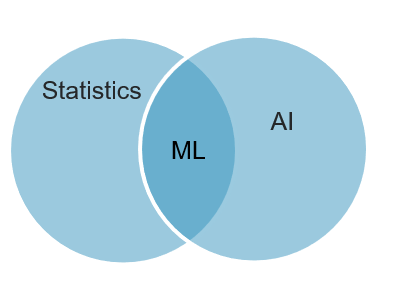
\includegraphics[width=0.95\textwidth]{pics/ml.png}
	\end{figure}
\end{columns}
\end{frame}

\begin{frame}
\frametitle{Lecture Overview}
\begin{block}{Chapters}
	\begin{enumerate}
		\item Basics and Linear Models
		\item Model Selection and Validation
		\item Trees
		\item Neural Nets
	\end{enumerate}
\end{block}

\begin{block}{Material}
	\url{https://github.com/mayer79/ml\_lecture}
\end{block}
\end{frame}

%=====================================================================
\section{Basics and Linear Models}
%=====================================================================

%=====================================================================
\subsection{Basics}
%=====================================================================

\begin{frame}
\frametitle{Before Modeling}
\begin{columns}
	\column{0.5\textwidth}
	\begin{itemize}
		\item Organization of data?
		\item Data types?
		\item Descriptive analysis
	\end{itemize}
	\begin{figure}
		
\includegraphics[width=0.6\textwidth]{pics/diamond.jpg}
	\end{figure}
	\column{0.5\textwidth}
	\begin{block}{Structure of diamonds data}
		\begin{figure}
			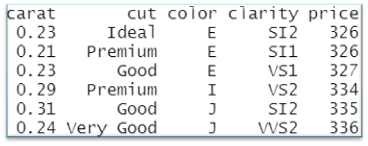
\includegraphics[width=0.95\textwidth]{pics/data_structure.png}
		\end{figure}
	\end{block}

	\begin{example}
	\end{example}
\end{columns}
\end{frame}

\begin{frame}
\frametitle{Statistical Models}
\begin{block}{Setting}
	\begin{itemize}
		\item Approximate \alert{response variable} $Y$ by function of \alert{covariates} $X_1,\dots,X_m$
		$$
			Y \approx f(X_1,\dots,X_m)
		$$
		\item Estimate unknown $f$ from data by $\hat f$.
		\item Use $\hat f$ for prediction and to investigate relationships.
		\item Postulate model equation
		$$
			\E(Y) = f(X_1, \dots, X_m)
		$$
		(we are often interested in means).
		\end{itemize}
	\end{block}
	
	\begin{block}{Remark}
	Other terms for response and covariates?
	\end{block}
\end{frame}

%=====================================================================
\subsection{Linear Regression}
%=====================================================================

\begin{frame}
\frametitle{Linear Regression}
\begin{itemize}
	\item 𝐸(𝑌)= 𝑓(𝑋_1, …, 𝑋_𝑚 )=𝛽_0+𝛽_1 𝑋_1+⋯+𝛽_𝑚 𝑋_𝑚
	Interpretation of coefficients 𝛽_𝑗? Ceteris Paribus!
	
	\item
\end{itemize}
\end{frame}

\begin{frame}
\frametitle{Linear Regression}
\begin{itemize}
	\item 
	\item
\end{itemize}
\end{frame}

\begin{frame}
\frametitle{Linear Regression}
\begin{itemize}
	\item 
	\item
\end{itemize}
\end{frame}

\begin{frame}
\frametitle{Linear Regression}
\begin{itemize}
	\item 
	\item
\end{itemize}
\end{frame}

\begin{frame}
\frametitle{Linear Regression}
\begin{itemize}
	\item 
	\item
\end{itemize}
\end{frame}

\begin{frame}
\frametitle{Linear Regression}
\begin{itemize}
	\item 
	\item
\end{itemize}
\end{frame}

%=====================================================================
\subsection{Generalized Linear Models}
%=====================================================================

%\begin{frame}
%    \frametitle{Introduction}
%    
%   	\begin{quotation}
%    	How to explain and interpret a given model, even if it seems a black box?		
%    \end{quotation}
%
%	\vfill
%	
%    \begin{block}{Answering this question is a key aspect of responsible ML}
%		\begin{enumerate}
%			\item Information for stakeholders
%			\item Detect problems in modeling process
%		\end{enumerate}
%    \end{block}
%
%	\vfill
%	
%	\begin{block}{XAI: e{\bf X}plainable {\bf A}rtificial {\bf I}ntelligence}
%		Collection of methods to explain and interpret models
%	\end{block}
%\end{frame}
%
%\begin{frame}
%    \frametitle{Scope and Taxonomy}
%    
%    \begin{block}{Scope}
%		XAI methods for structured data and {\bf bold} aspects below
%    \end{block}
%
%    \begin{block}{Taxonomy of explainability}
%		\begin{itemize}
%			\item {\bf Global} vs. local: Describe model as a whole or around an observation.
%			\item Model-specific vs. {\bf model-agnostic}: Some methods are tailored to specific model classes (linear regression, tree-based), others work for all types of models.
%			\item Intrinsic versus {\bf post-hoc}: Simple models like a linear regression can be interpreted intrinsically, while complex models require post-hoc analysis of fitted model. 
%		\end{itemize}
%    \end{block}
%
%	\begin{block}{Notes}
%		\begin{itemize}
%			\item Model-agnostic methods are always post-hoc
%			\item Model-agnostic methods can also be applied to intrinsically interpretable models
%			\item Won't make difference between ``explainable'', ``interpretable'', ``intelligible''
%		\end{itemize}
%	\end{block}
%\end{frame}
%
%\begin{frame}
%    \frametitle{XAI Outline}
%    
%    \begin{block}{1. Introduction}
%		\begin{itemize}
%			\item Notation
%			\item Non-life insurance pricing
%			\item Main example
%		\end{itemize}
%    \end{block}
%
%    \begin{block}{2. Explaining Models}
%    	\begin{itemize}
%    		\item Important post-hoc interpretation methods
%    		\item SHAP
%    		\item Improve GLM with the help of ML and XAI
%    	\end{itemize}
%    \end{block}
%    
%    \begin{block}{3. Improving Explainability}
%    	Improve intrinsic explainability of complex models by simplifying their structure
%    \end{block}    
%\end{frame}
%
%\begin{frame}
%    \frametitle{Notation}
%    \begin{block}{Basic modeling situation}
%    	\vspace{-1em}
%	    $$
%			T(Y\mid \bx) \approx m(\bx)
%		$$
%    	\vspace{-1em}
%	    \begin{itemize}
%	    	\item Distributional property $T(Y\mid \bx)$ of response $Y$
%	    	\item Model $m: \bx\in \R^p \mapsto \R$ of $p$-dim feature vector $\bx = (x^{(1)}, \dots, x^{(p)})^T$
%	    	\item $m$ estimated by $\hat m$ from training data by minimizing objective criterion
%	    	$
%	    	\sum_{i = 1}^n w_i L(\hat y_i, y_i) / \sum_{i = 1}^n w_i + \lambda \Omega(m)
%	    	$
%	    	\item $L$: loss/scoring function, ideally strictly consistent for $T$; $\lambda \Omega(m)$: optional penalty
%	    	\item $\boldsymbol w = (w_1, \dots, w_n)^T$: vector of (optional) case weights
%	    	\item $\boldsymbol y = (y_1, \dots, y_n)^T$: observed values of $Y$
%			\item $\boldsymbol{\hat y} = (\hat y_1, \dots, \hat y_n)^T$: predicted/fitted values $\hat y_i = \hat m(\bx_i)$
%	    	\item $\bx_1, \dots, \bx_n$: $n$ feature vectors; $x_i^{(j)}$: value of $j$-th feature of $i$-th observation
%	    \end{itemize}
%	\end{block}
%\end{frame}
%
%\begin{frame}
%	\frametitle{Examples of Models}
%	\begin{itemize}
%		\item Linear regression
%		\item Generalized linear models (GLM)
%		\item Generalized additive models (GAM)
%		\item Gradient boosted trees
%	\end{itemize}
%
%	\vfill
%	
%	Will peek into them as a quick refresher and to get used to notation
%\end{frame}
%
%\begin{frame}
%    \frametitle{Linear Regression}
%   	\begin{itemize}
%   		\item Model equation postulates
%   			$$
%   				\E(Y \mid \bx) = m(\bx) = \beta_o + \beta_1 x^{(1)} + \dots + \beta_p x^{(p)}
%   			$$
%   		\item $(\beta_o, \beta_1, \dots, \beta_p)^T \in \mathbb R^{p+1}$: parameter vector to be estimated
%   		\item Objective: Minimize sum of squared errors
%   			$$
%   				\sum_{i = 1}^n (y_i - \hat y_i)^2
%   			$$
%   			by linear least-squares
%   		\item Non-linear effects and interactions have to be added manually
%   		\item Penalized regression?
%   		\item Important extension: the generalized linear model (GLM)
%   	\end{itemize}
%\end{frame}
%
%\begin{frame}
%	\frametitle{Generalized Linear Model (GLM)}
%	\begin{itemize}
%		\item Model equation postulates
%			$$
%				\E(Y \mid \bx) = m(\bx) = g^{-1}(\eta(\bx)) = g^{-1}(\beta_o + \beta_1 x^{(1)} + \dots + \beta_p x^{(p)})
%			$$
%		\item $g^{-1}$: inverse link, $g$: link function, $\eta$: linear predictor
%		\item Parameters $\beta_j$ estimated by minimizing the (possibly weighted) {\em average deviance}
%			$$
%				\bar S(\hat m, D_{\text{train}}) = \sum_{i = 1}^n w_i S(\hat y_i, y_i) / \sum_{i = 1}^n w_i
%			$$
%			over training data $D_{\text{train}} = \{(y_i, w_i, \boldsymbol x_i), i = 1, \dots, n\}$
%	\end{itemize}
%
%	\begin{block}{(Unit) deviance}
%		\begin{itemize}
%			\item Distribution-specific measure: Poisson, Gamma, Bernoulli, normal, \dots
%			\item In our examples, we will often work with Poisson deviance
%				$
%					S(\hat y_i, y_i) = 2(y_i \log(y_i / \hat y_i) - (y_i - \hat y_i))
%				$
%		\end{itemize}
%	\end{block}
%\end{frame}
%
%\begin{frame}
%	\frametitle{Generalized Additive Model (GAM)}
%	\begin{itemize}
%		\item Extension of the GLM
%		\item Model equation assumes
%			$$
%				\E(Y \mid \bx) = m(\bx) = g^{-1}(\beta_o + f_1(x^{(1)}) + \dots + f_p(x^{(p)}))
%			$$
%		\item $f_j$: Sufficiently nice functions (some may be fully parameteric)
%		\item Estimated to minimize average deviance, e.g. using backfitting
%		\item Unlike a GLM, automatically accounts for non-linear effects
%		\item Like a GLM, a GAM can also include interaction effects
%	\end{itemize}
%\end{frame}
%
%\begin{frame}
%	\frametitle{Gradient Boosted Trees}
%	\begin{itemize}
%		\item Typical black-box $m$
%		\item Sum of decision trees
%		\item In contrast to GAM, automatically picks up interactions
%		\item Can optimize same objective criterion as GLMs/GAMs
%		\item Using a different model structure and a different optimization technique
%		\item Important implementations: LightGBM, XGBoost
%	\end{itemize}
%
%	\vfill
%	
%	Later, we will also work with neural nets
%\end{frame}
%
%\begin{frame}
%    \frametitle{Non-Life Insurance Pricing}
%    \begin{block}{Main task: Predict {\em pure premium} of insurance policy}
%    	\begin{itemize}
%    		\item Financial loss per year or per some other relevant exposure measure
%    		\item Used by company to optimize tariffs and to estimate expected future profit
%    		\item Predictions of statistical models fitted on historic data
%    	\end{itemize}
%    \end{block}   
%    
%   	\begin{block}{Discussion}
%		Why is it important to have good tariff?
%   	\end{block}
%\end{frame}
%
%\begin{frame}
%	\frametitle{Characterization of Insurance Policy}
%	\begin{columns}
%		\column{0.4\textwidth}
%		\begin{itemize}
%			\item $w > 0$: The exposure. Other quantities will refer to this
%			\item $N$: Number of claims
%			\item $C$: Total claim amount
%		\end{itemize}
%
%		\column{0.6\textwidth}
%		\begin{itemize}
%			\item $C / w$: Pure premium
%			\item $Y = N / w$: Claims frequency
%			\item $Z = C / N$: Severity = avg cost per claim
%			\item $\bx$: One or more risk characteristics
%		\end{itemize}		
%	\end{columns}
%		
%	\begin{example}[fictive motor third-part liability (MTPL) policies]
%		\begin{table}[!ht]
%			\centering
%			\begin{tabular}{|l|l|l|l|l|l|l|l|l|l|}
%				\hline
%				id & $w$ & $N$ & $C$ & $C/w$ & $Y$ & $Z$ & Driver's age & Horse power \\ \hline
%				1 & 1 & 0 & 0 & 0 & 0 & - & 28 & 80 \\ \hline
%				2 & 0.5 & 2 & 5000 & 10000 & 4 & 2500 & 20 & 250 \\ \hline
%				2 & 0.5 & 1 & 1000 & 2000 & 2 & 1000 & 21 & 250 \\ \hline
%			\end{tabular}
%		\end{table}
%	\end{example}
%
%	\begin{alertblock}{Remark}
%		Due to additivity of $w$, $N$, and $C$, these quantities can also be defined for multiple policies together, e.g., for the entire portfolio
%	\end{alertblock}
%\end{frame}
%
%\begin{frame}
%	\frametitle{Classic Pricing Models}
%	\begin{itemize}
%		\item Instead of creating a model for $\E(C / w \mid \bx)$, decompose pure premium
%		$$
%			C / w = (C / w) \cdot (N / N) = (N / w) \cdot (C / N) = Y  Z
%		$$
%		into product of frequency $Y$ and severity $Z$
%		\item Frequency model: $\E(Y \mid \bx) \approx m_Y(\bx)$
%		
%		$\rightarrow$ Poisson GLM with log link and case weights $w$
%		\item Severity model: $\E(Z \mid \bx) \approx m_Z(\bx)$
%	
%		$\rightarrow$ Gamma GLM with log link and case weights $N$, using only rows with $N>0$
%		\item Assuming conditional independence of $Y$ and $Z$, pure premium model is then
%		$
%			\E(C / w \mid \bx) \approx m_Y(\bx)  m_Z(\bx)
%		$
%	\end{itemize}
%	
%	\begin{block}{Alternative to GLMs}
%		\begin{itemize}
%			\item Replace GLMs by GAMs or modern ML techniques
%			\item Use same losses (deviance), weights, links
%		\end{itemize}
%	\end{block}
%\end{frame}
%
%\begin{frame}
%	\frametitle{More on Non-Life Insurance Pricing}
%	
%	\begin{itemize}
%		\item The severity model can use different features than the frequency model
%		\item The Gamma model with link is slightly biased $\rightarrow$ can be fixed by applying empirical multiplicative correction factor 
%		$$
%		c = \sum_{i = 1}^n y_i / \sum_{i = 1}^n \hat y_i
%		$$
%		calculated on the training data
%		\item Why using a log link for the Gamma model?
%		\item As an alternative to model claims frequency using case weights $w$, directly model claim counts $N$ without weights but using an offset of $\log(w)$
%		
%		$\rightarrow$ Same effects, different response, different evaluations
%	\end{itemize}
%\end{frame}
%
%\begin{frame}
%    \frametitle{Main Example}
%    \begin{example}[French motor third-part liability (MTPL) dataset]
%    	\begin{enumerate}
%    		\item Understand data
%    		\item Descriptive analysis
%    		\item Build claim frequency models
%	    \end{enumerate}
%    \end{example}
%
%	\begin{columns}
%		\column{0.5\textwidth}
%		\begin{block}{The models}
%			\begin{itemize}
%				\item Poisson GLM
%				\item Poisson GAM
%				\item Poisson gradient boosted trees
%			\end{itemize}
%		\end{block}
%	
%		\column{0.5\textwidth}
%		\begin{block}{Notes}
%			\begin{itemize}
%				\item Grouped train/test split
%				\item Model interpretation
%			\end{itemize}
%		\end{block}
%	\end{columns}
%\end{frame}
%
%%=====================================================================
%\section{XAI: Explaining Models}
%%=====================================================================
%
%\begin{frame}
%    \frametitle{Introduction}
%    \begin{columns}
%		\column{0.5\textwidth}
%		\begin{block}{Basic workflow to inspect and explain supervised learning model $m$}
%			\begin{enumerate}
%				\item Study model performance
%				\item Study feature importance
%				\item Study feature effects, ideally also interactions
%			\end{enumerate}
%		\end{block}
%		
%		\column{0.5\textwidth}
%		\begin{block}{Analysis result}
%			\begin{itemize}
%				\item Information gain
%				\item Reveal problems in model/data
%				\item Increase confidence in model and modeler
%			\end{itemize}
%		\end{block}
%    \end{columns}
%    
%    \begin{columns}
%	\column{0.5\textwidth}
%	\begin{block}{Focus}
%		Global, model-agnostic, post-hoc explainability
%	\end{block}
%	
%	\column{0.5\textwidth}
%	\begin{block}{Main references}
%		\begin{itemize}
%			\item Online book of Christoph Molnar
%			\item Tutorial (Mayer \& Lorentzen 2020)
%		\end{itemize}
%	\end{block}
%	\end{columns}    
%\end{frame}
%
%\begin{frame}
%	\frametitle{Chapter Outline}
%	\begin{enumerate}
%		\item Software
%		\item Performance
%		\item Excursion: grouped data
%		\item Variable importance
%		\item Effects
%		\item Global surrogate models
%		\item Improve linear models by XAI
%		\item SHAP
%	\end{enumerate}
%\end{frame}
%
%\begin{frame}
%    \frametitle{Software for Post-Hoc Interpretation}
%    \begin{columns}
%    	\column{0.5\textwidth}
%		\begin{block}{R}
%			\begin{itemize}
%				\item DALEX
%				\item iml
%				\item flashlight
%				\item SHAP: kernelshap, shapviz, fastshap
%				\item \dots
%			\end{itemize}
%		\end{block}
%
%    	\column{0.5\textwidth}		
%		\begin{block}{Python}
%			\begin{itemize}
%				\item scikit-learn inspect
%				\item DALEX
%				\item SHAP: shap
%				\item \dots
%			\end{itemize}
%		\end{block}
%	\end{columns}
%
%    \begin{columns}
%		\column{0.5\textwidth}
%		\begin{alertblock}{Programming workflow}
%			\begin{enumerate}
%				\item Build model
%				\item Create explainer object
%				\item Calculate and visualize results
%			\end{enumerate}
%		\end{alertblock}
%	
%		\column{0.5\textwidth}
%		\begin{example}
%		\end{example}
%	\end{columns}
%\end{frame}
%
%\begin{frame}
%    \frametitle{Performance}
%    \begin{itemize}
%    	\item Study one or more relevant performance measures
%    	\item Often: Average loss or function of it
%    	\item Gives valuable information
%    	\item Training versus test performance?	$\rightarrow$ assess overfitting/optimism
%    	\item Absolute and relative measures
%    \end{itemize}
%
%	\begin{block}{Also helps to detect problems}
%		\begin{itemize}
%			\item Is performance much lower than expected?
%				\begin{itemize}
%					\item Preprocessing errors
%					\item Missing key feature
%					\item Convergence problem
%				\end{itemize}
%			\item Is it much better?
%				\begin{itemize}
%					\item Data partitions really independent?
%					\item Leakage from response to feature?
%				\end{itemize}
%		\end{itemize}
%	\end{block}
%\end{frame}
%
%\begin{frame}
%	\frametitle{Example: Claims Frequency Models}
%	\begin{itemize}
%		\item Calculate weighted average Poisson deviance on test data:
%			$$
%				\bar S(\hat m, D_\text{test}) = \sum_{i = 1}^n w_i S(\hat y_i, y_i) / \sum_{i = 1}^n w_i
%			$$
%			with $S(\hat y_i, y_i) = 2(y_i \log(y_i / \hat y_i) - (y_i - \hat y_i))$
%		\item Relative deviance improvement (one of many ``pseudo R-squared'')
%			$$
%				1 - \frac{\bar S(\hat m, D_\text{test})}{\bar S(\hat m_\text{trivial}, D_\text{test})},
%			$$
%			where $\hat m_\text{trivial}(\bx) = \sum_{D_\text{train}} w_i y_i / \sum_{D_\text{train}} w_i$ is the intercept-only model with constant predictions ideally calculated on the training data	
%		\item Same on training data (why?)
%	\end{itemize}
%
%	\begin{example}
%	\end{example}
%\end{frame}
%
%\begin{frame}
%    \frametitle{Excursion: Grouped Data}
%    \begin{itemize}
%    	\item Flawed validation strategy $\rightarrow$ biased performance assessment
%    	\item Detailed knowledge of data and model required $\rightarrow$ difficult to detect
%    \end{itemize}
%
%	\begin{block}{Typical reason for flawed validation: Grouped data}
%		\begin{itemize}
%			\item Pricing data
%			\item Reserving: Models for ultimate claim amount
%			\item Customer analytics: Browser behaviour of online visitors
%			\item Banking: Financial transactions of clients
%		\end{itemize}
%	\end{block}
%
%    \begin{block}{Grouped splitting}
%		\begin{itemize}
%			\item Instead of random sampling of {\em rows}, we sample {\em groups}
%			\item All rows of a group go in same data partition
%			\item If ignored: Overfitting is being rewarded
%		\end{itemize}
%	\end{block}
%\end{frame}
%
%\begin{frame}
%	\frametitle{Example and Simulation}
%	\begin{example}[French MTPL]
%		\begin{itemize}
%			\item Model performance of GLM and boosted trees model without grouped splitting?
%			\item Impact on model tuning?
%		\end{itemize}
%	\end{example}
%
%	\begin{example}[Simulation]
%		\begin{itemize}
%			\item Random data
%			\item Linear regression and random forest
%			\item 80\%/20\% split
%			\item Increasing proportion of duplicated rows
%			\item Random split versus grouped split
%		\end{itemize}			
%	\end{example}
%\end{frame}
%
%\begin{frame}
%	\frametitle{More on Grouped Data}
%	\begin{itemize}
%		\item We used grouping structure to create clean data splits
%		\item Sometimes, one wants to also make use of within-group info in model
%		\item Panel data, time-series
%	\end{itemize}
%	
%	\vfill
%	
%	\begin{block}{Examples}
%		\begin{itemize}
%			\item Insurance of large vehicle fleets: credibility factors
%			\item Banking: Financial transactions of client
%		\end{itemize}
%	\end{block}
%
%	\vfill
%
%	Tricky to have clean validation strategy and to apply model correctly	
%\end{frame}
%
%\begin{frame}
%    \frametitle{Variable Importance}
%    \begin{enumerate}
%    	\item Information: Most/least important features?
%    	\item Challenge correctness of model
%    		\begin{itemize}
%	    		\item Results as expected or not?
%	    		\item Seemingly unimportant feature is top predictor $\rightarrow$ leakage?
%	    		\item Key features not among important features $\rightarrow$ preprocessing problem, not sufficient understanding of data or modeling situation?
%	    	\end{itemize}
%	\end{enumerate}
%	
%	\begin{block}{Model-specific variable importance measures}
%		\begin{itemize}
%			\item Linear model: normalized coefficients, test statistics etc.
%			\item Tree-based models: Split gain or split count		
%		\end{itemize}
%	\end{block}
%
%	\begin{block}{Model-agnostic measures}
%		\begin{itemize}
%			\item Permutation importance (Breiman 2001 for random forests)
%			\item SHAP feature importance
%		\end{itemize}
% 	\end{block}
%\end{frame}
%
%\begin{frame}
%	\frametitle{Permutation Importance}
%	Permutation importance of $j$-th feature $x^{(j)}$, data $D$, and performance measure $\hat S$:
%	$$
%		\text{PVI}(j, D) = \hat S(\hat m, D^{(j)}) - \hat S(\hat m, D)
%	$$
%	\vspace{-2em}
%	\begin{itemize}
%		\item $D^{(j)}$ is version of $D$ with randomly permuted values in $j$-th feature column
%		\item Read: How much $\hat S$ drops after shuffling column $j$? 
%		The higher, the more important. If 0, feature is unimportant
%	\end{itemize}
%	
%	\begin{block}{Algorithm to calculate $\text{PVI}(j, D)$ for all features}
%		\begin{figure}
%			\includegraphics[width=0.7\textwidth]{../r/figs/algo1_imp.png}
%			
%			\small{Source: Mayer and Lorentzen, 2020}
%		\end{figure}
%	\end{block}
%\end{frame}
%
%\begin{frame}
%	\frametitle{Remarks and Example}
%	\begin{columns}
%		\column{0.6\textwidth}
%		\begin{alertblock}{Remarks}
%			\begin{itemize}
%				\item Computationally cheap $\rightarrow$ repeat $m$ times
%				\item Model is never refitted
%				\item There is no formal definition of variable importance 
%				$\rightarrow$ inconsistency across methods
%				\item Different definitions of permutation importance
%				\item Strongly dependent features 
%				
%				$\rightarrow$ decorrelate or analyze together
%				\item Training or test data?
%			\end{itemize}
%		\end{alertblock}
%
%		\column{0.4\textwidth}	
%		\begin{example}[French MTPL]
%			\begin{itemize}
%				\item PVI using exposure-weighted average Poisson deviance
%				\item Hold-out data
%				\item Compare with tree-split gain
%			\end{itemize}
%		\end{example}
%	\end{columns}
%\end{frame}
%
%\begin{frame}
%    \frametitle{Effects}
%    \begin{block}{Study and understand feature effects is of key importance}
%    	\begin{itemize}
%	   		\item How does $m(\bx)$ change with $x^{(j)}$?
%	   		\item Often Ceteris Paribus: other components in $\bx$ fixed
%    	\end{itemize}
%
%    \end{block}
%
%    \begin{block}{Advantage of intrinsically interpretable models}
%	    \begin{itemize}
%	    	\item (Ceteris Paribus) effect of feature $x^{(j)}$ in a linear regression
%	    	$$
%	    	\E(Y \mid \bx) \approx m(\bx) = \beta_o +\beta_1 x^{(1)} + \dots + \beta_p x^{(p)}
%	    	$$
%	    	\item In an additive model
%	    	$$
%	    	\E(Y \mid \bx) \approx m(\bx) = \beta_o +f_1(x^{(1)}) + \dots + f_p(x^{(p)})
%	    	$$
%	    	\item In a black-box model?
%	    \end{itemize}
%	\end{block}
%\end{frame}
%
%\begin{frame}
%\frametitle{Methods}
%\begin{enumerate}
%	\item Individual conditional expectation (ICE)
%	\item Partial dependence
%	\item Classic diagnostic plots
%	\item Interactions?
%	\item Later: SHAP dependence plots
%\end{enumerate}
%\end{frame}
%
%\begin{frame}
%    \frametitle{Individual Conditional Expectation (ICE)}
%    \begin{block}{Basic thinking}
%	    \begin{itemize}
%	    	\item If $m$ is additive in $x^{(j)}$, the Ceteris Paribus effect of $x^{(j)}$ is the same for all observations 
%	    	$\rightarrow$ complete description of effect / full transparency
%	    	\item If complex interactions involved $\rightarrow$ approximate description only
%	    \end{itemize}
%	\end{block}
%	
%	\begin{block}{Idea (Goldstein et al., 2015)}
%		\begin{itemize}
%			\item Study Ceteris Paribus effect of $x^{(j)}$ for one observation
%			\item {\em ICE function} for feature $x^{(j)}$ of model $m$ and observation $\bx \in \R^p$
%			$$
%			\text{ICE}_j: v \in {\R} \mapsto m(v, \bx_{\setminus j})
%			$$
%			\item $\bx_{\setminus j}$ denotes all but the $j$-th component of $\bx$, which is replaced by $v$
%			\item {\em ICE curve} represents graph $(v, \text{ICE}_j(v))$ for grid of values $v \in \R$
%		\end{itemize}
%	\end{block}
%\end{frame}
%
%\begin{frame}
%	\frametitle{Simple Algorithm}
%	\begin{block}{Algorithm to calculate $ICE_j(v)$}
%		\begin{figure}
%			\includegraphics[width=0.8\textwidth]{../r/figs/algo2_ice.png}
%			
%			\small{Source: Mayer and Lorentzen, 2020}
%		\end{figure}
%	\end{block}
%\end{frame}
%
%\begin{frame}
%	\frametitle{ICE Plot: Visualize ICE curves of multiple observations}
%	\begin{example}
%	\end{example}
%
%	\begin{columns}
%		\column{0.5\textwidth}
%		\begin{block}{Notes}
%			\begin{itemize}
%				\item Curves with different shapes indicate interaction effects
%				\item Parallel curves $\rightarrow$ additivity in $x^{(j)}$
%				\item Centered ICE plots
%				\item Usually on link scale (why?)
%				\item ICE plots of higher dimension
%				\item Training versus test data
%			\end{itemize}
%		\end{block}
%			
%		\column{0.5\textwidth}
%		\begin{alertblock}{Pros and Cons}
%			\begin{itemize}
%				\item[+] Simple to compute
%				\item[+] Easy to interpret (Ceteris Paribus)
%				\item[+] Gives impression about interactions
%				\item[--] Suboptimal when Ceteris Paribus unnatural
%				\item[--] Does not show what variables are interacting
%			\end{itemize}
%		\end{alertblock}
%	\end{columns}
%\end{frame}
%
%\begin{frame}
%    \frametitle{Partial Dependence Plot PDP (Friedman 2001)}
%    \begin{itemize}
%    	\item Average of many ICE curves
%    	\item Ceteris Paribus effect of $x^{(j)}$ averaged over all interaction effects
%    \end{itemize}
%
%	\begin{block}{Definition}
%		\begin{itemize}
%			\item (Empirical) partial dependence function of feature $j$
%			$$
%			\text{PD}_j(v) = \frac{1}{n} \sum_{i = 1}^n \hat m(v, \bx_{i,\setminus j})
%			$$
%			\item $\bx_{i,\setminus j}$ feature vector of $i$-th observation without $j$-th component
%			\item PDP equals graph $(v, \text{PD}_j(v))$ for grid of values $v \in \R$
%			\item Sum runs over reference data (=?)
%		\end{itemize}
%	\end{block}
%\end{frame}
%
%\begin{frame}
%\frametitle{Algorithm}
%	\begin{block}{Calculate $PD_j(v)$ on grid of values for $v$}
%		\begin{figure}
%			\includegraphics[width=0.8\textwidth]{../r/figs/algo3_pd.png}
%			
%			\small{Source: Mayer and Lorentzen, 2020}
%		\end{figure}
%	\end{block}
%	\begin{example}	
%	\end{example}
%\end{frame}
%
%\begin{frame}
%	\frametitle{More on Partial Dependence}
%	\begin{columns}
%		\column{0.5\textwidth}
%		\begin{block}{Remarks}
%			\begin{itemize}
%				\item Two-dimensional PDP of $x^{(j)}$ and $x^{(k)}$:
%				$$
%				\text{PD}_{jk}(v_j, v_k) = \frac{1}{n} \sum_{i = 1}^n m(v_j, v_k, \bx_{i,\setminus \{j, k\}})
%				$$
%				\item Accumulated local effects (ALE)
%			\end{itemize}		
%		\end{block}
%	
%		\column{0.5\textwidth}
%		\begin{alertblock}{Pros and Cons}
%			\begin{itemize}
%				\item[+] Simple to compute
%				\item[+] Easy to interpret (Ceteris Paribus)
%				\item[--] Suboptimal when Ceteris Paribus unnatural
%				\item[--] No information about interactions
%			\end{itemize}
%		\end{alertblock}
%	\end{columns}
%\end{frame}
%
%\begin{frame}
%    \frametitle{Classic Diagnostic Plots}
%    \begin{columns}
%    	\column{0.5\textwidth}
%	    \begin{block}{Related plots}
%	    	\begin{enumerate}
%	    		\item Response versus covariate
%	    		
%	    		$\rightarrow$ Descriptive marginal effects
%	    		\item 
%	    		
%	    		Predicted versus covariate
%	    		
%	    		$\rightarrow$ Modeled marginal effects
%	    		\item Residual versus covariate: 
%	    		
%	    		$\rightarrow$ Bias assessment
%	    	\end{enumerate}
%	    \end{block}
%	    
%	    \column{0.5\textwidth}
%	   	\begin{alertblock}{Remarks}
%	   		\begin{itemize}
%	   			\item Small and large datasets
%	   			\item Binning of $x^{(j)}$
%	   			\item Training versus test data?
%	   			\item Relation to PDP?
%	   			\item Pros and Cons?
%	   		\end{itemize}
%		\end{alertblock}
%    \end{columns}
%
%	\vspace{1cm}
%	
%	\begin{example}
%	\end{example}
%\end{frame}
%
%\begin{frame}
%    \frametitle{Interaction Effects}
%    \begin{itemize}
%    	\item Interactions: Linear models versus black-box models
%    	\item ICE plot for $x^{(j)}$ gives impression of total interaction effects associated with $x^{(j)}$
%    \end{itemize}
%    
%    \begin{block}{Pairwise interaction strength: Friedman's $H$}
%    	$$
%    	H^2_{jk}=\frac{\sum_{i=1}^n \Big[\text{PD}_{jk}(x_i^{(j)}, x_i^{(k)}) - \text{PD}_{j}(x_i^{(j)}) - \text{PD}_{k}(x_i^{(k)})\Big]^2}{\sum_{i=1}^n \Big[\text{PD}_{jk}(x_i^{(j)}, x_i^{(k)})\Big]^2}
%    	$$
%    	\begin{itemize}
%    		\item Sums run over reference data
%    		\item Partial dependence functions are mean centered
%			\item Interpretation of $H^2$? When close to 0 or 1?
%			\item $H$ versus $H^2$
%    	\end{itemize}
%    \end{block}
%\end{frame}
%
%\begin{frame}
%	\frametitle{Absolute Interaction Strength}
%	Friedman's $H$ is a relative measure $\rightarrow$ absolute measure?
%		$$
%		\tilde H_{jk} = \sqrt{\frac{1}{n}\sum_{i=1}^n\Big[\text{PD}_{jk}(x_i^{(j)}, x_i^{(k)}) - \text{PD}_{j}(x_i^{(j)}) - \text{PD}_{k}(x_i^{(k)})\Big]^2}
%		$$
%		
%	\begin{block}{Remarks on $H$ and $\tilde H$}
%		\begin{itemize}
%			\item Find out {\em how} features are interacting?
%			
%			 $\rightarrow$ Two-dimensional PDP, stratified PDP, SHAP
%			\item Computational burden?
%			\item Usually, one works on link scale
%		\end{itemize}	
%	\end{block}
%	\begin{example}
%	\end{example}
%\end{frame}
%
%\begin{frame}
%    \frametitle{Global Surrogate Models}
%	\begin{block}{Idea}
%	\begin{itemize}
%	    \item Fit intrinsically interpretable model $m_I$ to predictions of $\hat m$
%		\item Usually a small decision tree
%		\item $\hat m_I$ is called (global) surrogate model for $\hat m$
%	    \item Objective function and R-squared of $\hat m_I$?
%	\end{itemize}
%	\end{block}
%	\begin{block}{Remarks}
%	\begin{itemize}
%	    \item Training or test data?
%	    \item Variable importances of $\hat m_I$?
%	\end{itemize}
%	\end{block}
%	\begin{example}
%	\end{example}
%\end{frame}
%
%\begin{frame}
%    \frametitle{Improve Linear Models by XAI}
%	\begin{block}{Workflow}
%	\begin{itemize}
%	    \item Build strong GLM by the help of ML and XAI
%	    \item Why not directly use ML model?
%	\end{itemize}
%	\end{block}
%	\begin{block}{Compare XAI aspects}
%	\begin{enumerate}
%	    \item Performance: Difference between GLM and ML model large or small?
%	    \item Variable importance: Similar features important?
%		\item Main effects: Similar or not? $\rightarrow$ Change representation in GLM
%		\item Interaction effects: Add strong meaningful interactions to GLM
%	\end{enumerate}
%	\end{block}
%	\begin{example}
%	\end{example}
%\end{frame}
%
%\begin{frame}
%    \frametitle{SHAP: SHapley Additive exPlanations}
%	\begin{columns}
%        \column{0.3\textwidth}
%		\begin{itemize}
%			\item Local explanations
%			\item Basic idea of SHAP?
%			\item LIME
%		\end{itemize}
%		
%        \column{0.7\textwidth}
%	    \begin{figure}
%	        \includegraphics[width=0.99\textwidth]{figs/shap_waterfall.jpg}
%	    \end{figure}
%	\end{columns}
%\end{frame}
%
%\begin{frame}
%    \frametitle{Shapley Values}
%	\begin{block}{Setting}
%		\begin{itemize}
%			\item $\M$: Set of $p = |\M|$ players 
%			\item Playing cooperative game with numeric payoff
%			\item Contribution of subset $\L \subseteq \M$ of players measured by function $v: \L \mapsto \mathbb R$
%		\end{itemize}
%	\end{block}
%	\begin{block}{Question}
%		How to distribute payoff fairly among the players?
%	\end{block}
%	\begin{block}{Answer by Shapley (1953)}
%		Player $j$ should receive ``Shapley value'' = weighted average contribution
%		$$
%		  \phi_j(v) = \phi_j = \sum_{\L \subseteq \M \setminus\{j\}} \underbrace{\frac{|\L|!(p - |\L| - 1)!}{p!}}_{\text{Shapley weight}} (\underbrace{v(\L \cup \{j\}) - v(\L)}_{\text{Contribution of player } j}), \ \ j = 1, \dots, p.
%		$$
%	\end{block}
%\end{frame}
%
%\begin{frame}
%    \frametitle{Fairness}
%	$\phi_j$ averages the $p$ average contributions of player $j$ to coalitions of size $0 \le |\L| \le p-1$:
%	$$
%	  \text{Shapley weight} = \frac{|\L|!(p - |\L| - 1)!}{p!} = \frac{1}{p}\frac{1}{{p-1 \choose |\L|}}.
%	$$
%	Link to permutations?
%	
%	\begin{block}{Shapley values are only way to distribute total winnings fairly in the sense:}
%		\begin{enumerate}
%			\item Efficiency: $v(\M) = \sum_{j = 0}^p \phi_j$, where $\phi_o = v(\emptyset)$ denotes non-distributed payoff
%			\item Symmetry: If $v(\L \cup \{i\}) = v(\L \cup \{j\})$ for every $\L \subseteq \M \setminus\{i, j\}$, then $\phi_i = \phi_j$
%			\item Dummy player: If $v(\L \cup \{j\}) = v(\L)$ for all coalitions $\L \subseteq \M \setminus\{j\}$, then $\phi_j = 0$
%			\item Linearity: Consider two cooperative games with gain functions $v$ and $w$. Then, $\phi_j(v + w) = \phi_j(v) + \phi_j(w)$ and $\phi_j(\alpha v) = \alpha \phi_j(v)$ for all $1 \le j \le p$ and $\alpha \in \mathbb R$
%		\end{enumerate}
%	\end{block}
%\end{frame}
%
%
%\begin{frame}
%    \frametitle{Shapley Values in Statistics and ML}
%	\begin{block}{Early idea}
%		Lipovetsky and Conklin (2001): Fair decomposition of {\em R-squared} in linear regression
%	\end{block}
%	\begin{block}{Nowadays: Štrumbelj and Kononenko (2010, 2014), Lundberg and Lee (2017)}
%		\begin{itemize}
%			\item Decompose {\em predictions} fairly into
%			$
%				m(\bx) = \phi_o + \sum_{j = 1}^p \phi_j, \quad \phi_o = \E(m(\bX))
%			$
%			\item Fair only if $\phi_j$ are Shapley values
%			\item Natural contribution function: $v(\L) = m(\bx_\L)$, $\bx_\L$ are components in $\L \subseteq \M$
%			\item But: Features cannot be turned off in $m(\bx_\L)$ $\rightarrow$ use statistics to estimate it
%		\end{itemize}
%	\end{block}
%	\begin{block}{Situations where no estimation is required}
%		\begin{itemize}
%			\item $p=1$: Then $\phi_1 = m(\bx) - \phi_o$
%			\item Linear regression without correlations: 
%			$$
%				m(\bx) = \underbrace{\beta_0}_{\phi_o} + \underbrace{\beta_1 x^{(1)}}_{\phi_1} + \dots + \underbrace{\beta_p x^{(p)}}_{\phi_p}
%			$$
%		\end{itemize}
%	\end{block}
%\end{frame}
%
%\begin{frame}
%	\frametitle{How to Estimate Contribution Function}
%	\begin{block}{Controversy in estimating $m(\bx_\L)$}
%		\begin{itemize}
%			\item Statistically natural: Conditional expectation $\E(m(\bX \mid \bx_\L))$
%			\item Causal inference prefers marginal expectations: $\E_{\bX_{\M \setminus \L}}(m(\bX))$
%		\end{itemize}
%	\end{block}
%
%	\begin{block}{Algorithms (from slow to fast)}
%		\begin{enumerate}
%			\item Monte Carlo sampling: For each $j$ and many $\L$, contributions $v(\L\cup\{j\}) - v(\L)$ are evaluated using marginal expectations and then plugged into Shapley's Eq.
%			\item Kernel SHAP: For many $\L$, evaluates $v(\L)$ using marginal expectations. Then use regression to get all Shapley values without plugging into Shapley's Eq.
%			\item TreeSHAP: Uses properties of trees to directly calculate $v(\L)$ for all $\L\subseteq \M$ and then plugging into Shapley's Eq.
%		\end{enumerate}
%	\end{block}
%	\begin{example}
%	\end{example}
%\end{frame}
%
%\begin{frame}
%    \frametitle{From Local to Global Explanations}
%   	\begin{block}{Notation}
%	   	\begin{itemize}
%	   		\item $X$: $(n \times p)$ feature matrix with elements $x_{ij}$, $1 \le i \le n$, $1 \le j \le p$
%	   		\item $\Phi$: $(n \times p)$ matrix of SHAP values with elements $\phi_{ij}$
%	   		\item $\phi_o = \frac{1}{n} \sum_{i = 1}^n \hat m(\bx_i)$
%	   		\item $\hat m(\bx_i) = \phi_o + \sum_{j = 1}^p \phi_{ij}$ for $n$ feature vectors $\bx_i$
%	   	\end{itemize}
%    \end{block}
%	\begin{block}{Strategy to understand model as a whole}
%		\begin{itemize}
%			\item SHAP feature importance: $I_j=\frac{1}{n}\sum_{i=1}^n|\phi_{ij}|$
%			\item SHAP dependence plots: $\{(x_{ij}, \phi_{ij}), 1 \le i \le n\}$
%			\item Interactions: Use $x_{ik}, k \ne j$ to add color to SHAP dependence plot (alternative?)
%		\end{itemize}
%	\end{block}
%	\begin{exampleblock}{Examples}
%		Each aspect separately and full analysis
%	\end{exampleblock}
%\end{frame}
%
%\begin{frame}
%	\frametitle{SHAP Analysis to Improve Linear Model}
%	\begin{block}{Revisit our strategy}
%		\begin{itemize}
%			\item A lot of info on a ML black-box $m$ can be generated very quickly
%			\item Use it to build strong GLM
%		\end{itemize}
%	\end{block}
%	\begin{example}
%	\end{example}
%
%	\begin{block}{Remember}
%		SHAP has a solid theoretical foundation. In practice, some of it is lost because statistics is not mathematics.
%	\end{block}
%\end{frame}
%
%
%%=====================================================================
%\section{XAI: Improving Explainability}
%%=====================================================================
%
%\begin{frame}
%    \frametitle{Introduction}
%    \textquote[Lundberg and Lee, 2017]{The best explanation of a simple model is the model itself}
%    
%    \begin{block}{Two main strategies in XAI}
%    	\begin{itemize}
%    		\item Model is black-box $\rightarrow$ interpret it post-hoc
%    		\item Make model less opaque / improve intrinsic explainability
%    	\end{itemize}
%	\end{block}
%	
%	\begin{block}{Basic hierarchy of intrinsic explainability}
%		\begin{enumerate}
%			\item Linear additive models (like GLMs)
%			\item Additive models (like GAMs)
%			\item Black-box models (like boosted trees or neural nets)
%		\end{enumerate}
%	\end{block}
%    
%    \begin{alertblock}{Note}
%    	\begin{itemize}
%    		\item To link or not?
%    		\item Single decision tree
%    	\end{itemize}
%    \end{alertblock}
%\end{frame}
%
%\begin{frame}
%	\frametitle{Boundaries are Blurred}
%	\begin{exampleblock}{Examples}
%		\begin{itemize}
%			\item GLMs can have non-linear effects
%			\item GLMs and GAMs can have interactions
%			\item A complex GLM can be (almost) as black-box as a boosted trees model
%			\item \alert{Boosted trees models can have all or some features additive}
%			\item \alert{Neural nets can have all or some features additive}
%		\end{itemize}
%	\end{exampleblock}
%	
%	\begin{block}{Partly additive models = Additive with (possibly complex) interactions}
%		\begin{itemize}
%			\item Additive time effects: $m(\bx) = f(\text{Time}) + f'(\text{other features})$
%			\item Additive gender effects: $m(\bx) = f(\text{Gender}) + f'(\text{other features})$
%			\item Additive model with non-additive location effects: $m(\bx) = f_1(x^{(1)}) + \dots + f_{p_1}(x^{(p_1)}) + f(\text{location features})$
%		\end{itemize}
%	\end{block}
%\end{frame}
%
%\begin{frame}
%	\frametitle{Chapter Outline}
%	\begin{block}{Structuring boosted trees}
%		\begin{itemize}
%			\item Additive models
%			\item Partly additive models
%			\item Monotonicity
%		\end{itemize}
%	\end{block}
%	
%	\begin{block}{Structuring neural nets}
%		\begin{itemize}
%			\item Additive models
%			\item Partly additive models
%		\end{itemize}
%	\end{block}
%	
%	\begin{block}{Tune boosted trees models}		
%		Only if time
%	\end{block}
%\end{frame}
%
%\begin{frame}
%    \frametitle{Structuring Boosted Trees}
%	\begin{block}{Interpreting boosted trees models}
%		\begin{itemize}
%			\item Single decision trees $m_k$ are simple to interpret
%			\item Boosted trees $m$ are sums of $K$ decision trees
%				$$
%				m(\boldsymbol x) = m_1(\boldsymbol x) + \dots + m_K(\boldsymbol x)
%				$$
%			\item Interpretation of $m$ only post-hoc
%		\end{itemize}
%	\end{block}
%
%    \begin{block}{Will investigate two ways to structure boosted trees}
%    	\begin{enumerate}
%			\item Additive boosted trees
%			\item Partly additive boosted trees
%    	\end{enumerate}
%    Both are extremely useful in practice
%    \end{block}
%\end{frame}
%
%\begin{frame}
%    \frametitle{Additive Boosted Trees}
%    \begin{block}{What is a tree stump?}
%		\begin{itemize}
%			\item Decision tree $m_k$ with only one split
%			\item Can be written as $m_k(\bx) = v_1 + (v_2 - v_1)\mathbb I(x^{(j)} \le s)$; \ ($v_1$, $v_2$, $s=$?)
%		\end{itemize}
%    \end{block}
%
%	\begin{block}{Boosted tree stumps are additive models}
%		\begin{itemize}
%			\item $m(\bx) = \beta_o + f_1(x^{(1)}) + \dots + f_p(x^{(p)})$
%			\item $f_j$, $1 \le j \le p$, are piecewise constant functions derived from $m_k$
%		\end{itemize}
%	\end{block}
%
%	\begin{figure}
%		\includegraphics[width=0.9\textwidth]{../r/figs/tree_additive.png}
%	\end{figure}
%\end{frame}
%
%\begin{frame}
%	\frametitle{More on Boosted Tree Stumps}
%	\begin{itemize}
%		\item Additivity $\rightarrow$ full description of feature effects via ICE/PDP
%		\item SHAP dependence plot? (Mayer 2022)
%		\item Discussion: Pros and cons versus classic GAM?
%		\item References: Lou et al. (2012), Nori et al. (2019)
%	\end{itemize}
%
%	\vfill
%
%	\begin{example}
%	\end{example}
%\end{frame}
%
%\begin{frame}
%    \frametitle{Partly Additive Boosted Trees}
%   	\begin{itemize}
%   		\item Grow trees of depth $m = 2$ $\rightarrow$ pairwise interactions
%   		\item Partly additive model via {\em interaction constraints} (Lee et al., 2015)
%   	\end{itemize}
%   
%   	\begin{block}{Interaction constraints}
%		\begin{itemize}
%			\item $IC = \{F_1, \dots, F_M\}$
%			\item Each $F_m \subseteq \mathcal M$ is feature subset allowed to interact
%		\end{itemize}
%   	\end{block}
%   
%   	\begin{block}{How do they work?}
%   	\begin{itemize}
%   		\item Consider a decision tree
%   		\item Rule: Each split considers features only from those $F_m$ that contain all previous split variables of the branch.
%   		\item Thus, each branch will use features only from one $F_m \in IC$.
%   		\item Translates to tree and tree ensemble.
%   	\end{itemize}
%   \end{block}
%\end{frame}
%
%\begin{frame}
%	\frametitle{Partly Additive Models via Interaction Constraints}
%	\begin{block}{How to set $IC$ so that model is additive in $j$-th feature?}
%		\begin{itemize}
%			\item $F_m = \{x^{(j)}\}$ for some $m$
%			\item $x^{(j)} \notin F_k, \ k \ne m$		
%		\end{itemize}
%	\end{block}
%	
%	\begin{example}
%	$
%		IC = \{\{\text{DrivAge}\}, \{\text{logDensity}\}, \{\text{PolicyRegion}\}, \{\text{VehAge}, \text{Brand}, \text{Gas}, \text{Power}\}\}
%	$	
%	\end{example}
%
%   	\begin{figure}
%		\includegraphics[width=0.85\textwidth]{../r/figs/tree_partly_additive.png}
%	\end{figure}
%	
%\end{frame}
%\begin{frame}
%\frametitle{More on Interaction Constraints}
%	\begin{itemize}
%		\item If all elements in $IC$ are disjoint, each tree uses features from only one $F_m$
%		\item How is the first split variable determined?
%		\item $IC = \{\{x^{(1)}\}, \dots, \{x^{(p)}\}\}$ gives additive model:
%		\begin{figure}
%			\includegraphics[width=0.8\textwidth]{../r/figs/tree_additive_ic.png}
%		\end{figure}
%		\item Difference to boosted tree stumps?
%	\end{itemize}
%\end{frame}
%
%\begin{frame}
%    \frametitle{Monotonic Constraints}
%    \begin{columns}
%    	\column{0.35\textwidth}
%    	\begin{itemize}
%    		\item Monotonicity of $m(\bx)$ in feature $j$ is another aspect of interpretability
%    		\item Violated natural monotonicity can have dramatic impact on trustworthiness
%    		\item Examples in car {\em collision} models?
%    		\item Simple to implement for decision trees!
%    	\end{itemize}
%    	
%    	\column{0.65\textwidth}
%	    \begin{figure}
%	    	\includegraphics[width=1\textwidth]{../r/figs/monotonic.jpg}
%	    	\caption{Aim: monotone decreasing predictions in vehicle age}
%	    \end{figure}
%	\end{columns}
%\end{frame}
%
%\begin{frame}
%	\frametitle{More on Monotonic Constraints}
%	\begin{itemize}
%		\item Monotonicity translates to tree ensembles
%		\item Be careful when imposing monotonicity (why?)
%		\item Can help to reduce wiggliness of effect
%		\item Monotonicity for other model classes like GLMs, GAMs, neural nets?
%		\item Monotonicity and outlying feature values
%	\end{itemize}
%
%	\vfill
%	
%	\begin{example}
%	\end{example}
%\end{frame}
%
%\begin{frame}
%    \frametitle{Structuring Neural Nets}
%    \begin{columns}
%    	\column{0.65\textwidth}
%		\begin{block}{Swiss army knife of ML: Neural nets can}
%		\begin{itemize}
%			\item mimic GLMs and GAMs,
%			\item learn interactions and non-linear effects,
%			\item fit data larger than RAM (e.g. images, videos),
%			\item learn ``online'',
%			\item use multidimensional input and output,
%			\item use input and output of mixed dimensionality,
%			\item fit models with millions of parameters,
%			\item perform non-linear dimension reduction,
%			\item \dots
%		\end{itemize}
%		\end{block}
%	
%	    \column{0.35\textwidth}
%	    \begin{block}{How to create}
%	    	\begin{enumerate}
%	    		\item linear,
%	    		\item complex,
%	    		\item additive, and
%	    		\item partly additive
%	    	\end{enumerate}
%	    	neural nets?
%    	\end{block}
%    \end{columns}
%\end{frame}
%
%\begin{frame}
%	\frametitle{Some Notes on Neural Nets}
%	\begin{itemize}
%		\item Why haven't we worked with neural nets so far?
%		\item Neural nets versus boosted trees?
%		\item References?
%		\item TensorFlow, PyTorch, Keras
%		\item Keras: sequential versus functional API
%		\item Keras in R
%	\end{itemize}	
%\end{frame}
%
%\begin{frame}
%    \frametitle{A Simple Neural Net: GLM}
%    \begin{columns}
%	\column{0.5\textwidth}
%	\begin{block}{Some slang}
%		\begin{itemize}
%			\item Input and output layer?
%			\item Nodes and node values?
%			\item Fully connected / dense layer			
%			\item Exponential activation function
%		\end{itemize}
%	\end{block}
%	
%	\column{0.5\textwidth}
%    \begin{figure}
%    	\includegraphics[height=0.85\textheight]{figs/nn_glm.jpg}
%    \end{figure}
%	\end{columns}
%\end{frame}
%
%\begin{frame}
%	\frametitle{Example and Parameter Estimation}
%	\begin{block}{Parameters estimated by (mini-batch) gradient descent with backpropagation}
%		\begin{enumerate}
%			\item Initialization: Randomly set parameters.
%			\item Forward step: Calculate predictions and their (total) loss of a {\em batch}
%			\item Backward step: Change parameters in the negative directions of the gradient of the loss to make loss smaller on that batch
%			\item Iterate Steps 2--3 for one epoch, i.e., until the full training data has been used
%			\item Iterate Step 4 until validation performance stops improving
%		\end{enumerate}
%	\end{block}
%
%	\begin{example}
%		\begin{itemize}
%			\item Naive numeric representation of categoricals
%			\item Callbacks?
%			\item Feature scaling (why? how?)
%		\end{itemize}
%	\end{example}
%\end{frame}
%
%\begin{frame}
%    \frametitle{More Complex Models}
%    \begin{columns}
%    	\column{0.4\textwidth}
%    	\begin{block}{Some additional slang}
%			\begin{itemize}
%				\item Hidden layers
%				\item Representational learning
%				\item Activation functions: 
%				
%				two purposes
%				\item How to choose architecture?
%				\item How to choose number of parameters/weights?
%			\end{itemize}
%    	\end{block}
%    	
%    	\begin{example}
%    		\begin{itemize}
%    			\item Three hidden layers
%    			\item 561 parameters
%    		\end{itemize}
%	    \end{example}
%    	
%    	\column{0.6\textwidth}
%    	\begin{figure}
%    		\includegraphics[width=1\textwidth]{figs/nn_complex.jpg}
%    	\end{figure}
%    \end{columns}
%\end{frame}
%
%\begin{frame}
%    \frametitle{Additive Neural Nets (Agarwal et al. 2020)}
%    
%    \begin{columns}
%	   	\column{0.6\textwidth}
%	   	\begin{itemize}
%	   		\item Represent each feature by single-output net
%	   		\item Directly connected to output layer
%	   		\item Linear components?
%	   		\item Unordered categorical features?
%	   	\end{itemize}
%   	
%	   	\begin{example}
%	   		\begin{itemize}
%	   			\item `VehBrand', `PolicyRegion': 1-D embedding
%	   			\item `VehGas' and `logDensity': Scaled and represented by linear function
%	   			\item Rest: Scaled and represented by small net each
%	   			\item Almost same structure as our original GAM
%	   		\end{itemize}
%	   	\end{example}	   	
%   	
%	   	\column{0.4\textwidth}
%	    \begin{figure}
%	    	\includegraphics[height=0.8\textheight]{figs/nn_additive.jpg}
%	    \end{figure}
%    	\vspace{-1em}
%	    \tiny{Source: Fig 1a in https://www.mdpi.com/1911-8074/15/5/193}
%    \end{columns}
%\end{frame}
%
%\begin{frame}
%    \frametitle{Partly Additive Models}
%    \begin{columns}
%    	\column{0.5\textwidth}
%    	\begin{itemize}
%    		\item Pairwise interactions
%			\item Partly additive model
%    		\item Use case in geographic modeling
%    		\item Make model additive in driver features?
%    	\end{itemize}
%    	
%		\begin{example}
%			\begin{itemize}
%				\item `logDensity': Scaled and represented as a linear function
%				\item `DrivAge': Scaled and represented by a small sub-network
%				\item `PolicyRegion': 1-D embedding
%				\item Vehicle features: sub-network with different inputs and five outputs	
%			\end{itemize}
%		\end{example}
%    	
%    	\column{0.5\textwidth}
%	    \begin{figure}
%	    	\includegraphics[height=0.8\textheight]{figs/nn_partly_additive.jpg}
%	    \end{figure}
%       	\vspace{-1em}
%	    \tiny{Source: Fig 1b in https://www.mdpi.com/1911-8074/15/5/193}
%    \end{columns}
%\end{frame}
%
%\begin{frame}
%    \frametitle{Excursion: Tuning Boosted Trees}
%    \begin{block}{Model tuning in general}
%		\begin{itemize}
%			\item How to choose hyperparameters of ML models?
%			\item Each model class (GLMs, GAMs, random forests, boosted trees, neural nets, \dots) has specialities that should be respected
%			\item Examples?
%		\end{itemize}
%    \end{block}
%    
%    \begin{columns}
%    	\column{0.5\textwidth}
%		\begin{block}{Why focussing on boosted trees?}
%		\begin{itemize}
%			\item Usually among best performing models for tabular data
%			\item Boosting + SHAP $\rightarrow$ strong GLMs
%			\item It needs some training
%		\end{itemize}
%		\end{block}
%	
%	  	\column{0.5\textwidth}		
%		\begin{block}{Aspects}
%			\begin{enumerate}
%				\item Objective and evaluation metric
%				\item Number of boosting rounds
%				\item Learning rate
%				\item Further parameters
%			\end{enumerate}
%		\end{block}
%    \end{columns}
%\end{frame}
%
%\begin{frame}
%	\frametitle{Objective and Metric}
%	\begin{block}{Ideal choice of loss function}
%		\begin{itemize}
%			\item Meaningful for task
%			\item Strictly consistent for target functional $T$
%		\end{itemize}
%	\end{block}
%
%	\begin{block}{Translation to objective and metric}
%		\begin{itemize}
%			\item Objective: average loss on training data (plus regularization) used for model training
%			\item Evaluation metric: average (cross-)validation loss used for model comparison and selection
%		\end{itemize}
%	\end{block}
%
%	\begin{Example}
%	\end{Example}
%\end{frame}
%
%\begin{frame}
%	\frametitle{Number of Boosting Rounds}
%	\begin{block}{Very important to select reasonable number of boosting rounds}
%		\begin{itemize}
%			\item Boosting round = tree
%			\item Too few rounds $\rightarrow$ underfitting
%			\item Too many rounds $\rightarrow$ overfitting
%			\item Heavily depends on choice of other parameters, thus difficult to choose
%		\end{itemize}
%	\end{block}
%
%	\begin{block}{``Early stopping'' as standard solution}
%		\begin{itemize}
%			\item How does it work?
%			\item Why is it so convenient?
%		\end{itemize}
%	\end{block}
%\end{frame}
%
%\begin{frame}
%	\frametitle{Learning Rate}
%	\begin{itemize}
%		\item Weight of each tree in final model
%		\item Often between wide range of 1 and 0.005
%		\item Good value heavily depends on number of boosting rounds
%		\item Trick: select it so that early stopping ends after $100-1000$ trees (why?)
%		\item Halving the number of trees means doubling the learning rate for comparable performance
%	\end{itemize}
%\end{frame}
%
%\begin{frame}
%	\frametitle{Regularization Parameters}
%	\begin{columns}
%		\column{0.5\textwidth}
%		\begin{block}{Additional parameters to select}
%			\begin{itemize}
%				\item number of leaf nodes
%				\item tree depth
%				\item loss penalties
%				\item different types of subsampling rates
%				\item \dots
%			\end{itemize}
%		\end{block}
%		
%		\column{0.5\textwidth}
%		\begin{block}{Choose them by (cross-)validation}
%			\begin{itemize}
%				\item One by one
%				\item Grid-search
%				\item Random search
%			\end{itemize}
%		\end{block}
%	\end{columns}
%	
%	\vfill
%	
%	\begin{alertblock}{Note}
%		\begin{itemize}
%			\item Early-stopping often compensates for suboptimal choice of other parameters
%			\item Very different parameter combinations may lead to similar performance
%		\end{itemize}
%	\end{alertblock}
%\end{frame}
%
%\begin{frame}
%\frametitle{Overall Strategy}
%	\begin{block}{Three steps}
%		\begin{enumerate}
%			\item Choose strictly consistent and meaningful loss for functional $T$ 
%			
%			$\rightarrow$ objective and evaluation metric
%			\item Choose learning rate to get $100-1000$ trees with early stopping
%			\item Select remaining parameters manually or by random search via (cross-)validation
%		\end{enumerate}
%	\end{block}
%
%	\begin{block}{Simplification}
%		When to skip expensive Step 3?
%	\end{block}
%
%	\begin{example}
%		\begin{itemize}
%			\item French MTPL
%			\item Speciality: grouped partitions
%		\end{itemize}
%	\end{example}
%\end{frame}

\end{document}